\documentclass[12pt]{article}

\usepackage[utf8]{inputenc}
\usepackage[serbian]{babel}
\usepackage{graphicx}
\usepackage[hidelinks]{hyperref}
\usepackage{csquotes}
\usepackage[backend=biber, style=numeric, sorting=none]{biblatex}
\usepackage{float}

\usepackage{geometry}
\geometry{
    a4paper,
    left=25mm,
    top=25mm,
    right=25mm,
    bottom=25mm
}
\addbibresource{literatura.bib}

\begin{document}

\begin{titlepage}
\newcommand{\HRule}{\rule{\linewidth}{0.5mm}}
\center

\textsc{\LARGE Matematički fakultet, Univerzitet u Beogradu}\\[1.5cm]
\textsc{\Large Računarstvo i društvo}\\[0.5cm]
\textsc{\large Seminarski rad}\\[0.5cm]

\HRule \\[0.4cm]
{ \huge \bfseries Analiza sistema Gotham: Integracija velikih podataka i etika AI u vojnim i obaveštajnim sistemima}\\[0.4cm]
\HRule \\[1.5cm]

\begin{minipage}{0.4\textwidth}
\begin{flushleft} \large
\emph{Student:}\\
Nemanja Badrić 295/2021
\end{flushleft}
\end{minipage}
~
\begin{minipage}{0.4\textwidth}
\begin{flushright} \large
\emph{Mentor:} \\
Dr Sana Stojanović Đurđević\\
Katedra za računarstvo i informatiku
\end{flushright}
\end{minipage}\\[1.5cm]

{\large 2026}\\[2cm]

\vfill
\end{titlepage}

\newpage
\tableofcontents
\newpage

\section{Uvod}

Savremeno ratovanje i obaveštajni rad suočavaju se sa izazovom obrade ogromne količine heterogenih podataka. Sistem Palantir Gotham prvobitno je dizajniran nakon terorističkih napada 11. septembra kako bi se rešio problem izolovanih baza podataka (eng. \textit{data silos}) i katastrofalnih propusta u obaveštajnom radu \cite{wei2024brief}. Danas se Gotham razvio u sveobuhvatan okvir za donošenje globalnih odluka, koji integriše masovne i heterogene skupove podataka, centralizovane u takozvanim jezerima podataka (eng. \textit{Data lakes}), i transformiše ih u jedinstvenu operativnu sliku \cite{wei2024brief}.

Iako ovakvi sistemi donose ogromnu stratešku prednost, oni iz korena menjaju način na koji se upravlja vojnim operacijama \cite{wei2024brief}. U tradicionalnom vojnom procesu donošenja odluka, poznatom kao OODA ciklus (eng. \textit{Observe, Orient, Decide, Act}), sistemi mašinskog učenja danas sve više preuzimaju ključnu ulogu u samom odlučivanju \cite{wei2024brief}. Oslanjanje na veštačku inteligenciju u ovom procesu dovodi do toga da se gubi jasna granica između onoga što je svesna ljudska odluka i onoga što je mašina autonomno sprovela u delo \cite{woodcock2024human}. Ovo dovodi do složenih etičkih pitanja o tome kako algoritamski sistemi podrške u odlučivanju (eng. \textit{Decision-Support Systems - DSS}) utiču na ljudsku odgovornost i procenu proporcionalnosti napada prema Međunarodnom humanitarnom pravu \cite{woodcock2024human}.

Pored vojne etike, sve veća integracija ovakvih platformi otvara i ozbiljna pitanja o privatnosti i bezbednosti. Privatne tehnološke kompanije se danas sve više integrišu u državne i vojne strukture, preuzimajući zadatke koji su tradicionalno bili isključivo u nadležnosti države \cite{carnegie2024private}.
Ovo stvara ozbiljan problem sa odgovornošću, jer država gubi direktan uvid i kontrolu nad tim kako zatvoreni algoritmi privatnih kompanija obrađuju osetljive podatke i donose zaključke na terenu \cite{ulbricht2024palantir}.

Cilj ovog seminarskog rada je detaljna analiza arhitekture sistema Palantir Gotham, sa posebnim osvrtom na to kako integracija velikih podataka oblikuje etiku u vojnoj primeni i stvara nove bezbednosne pretnje po privatnost na internetu. Rad će prvo prikazati tehničku osnovu sistema kroz koncept dinamičke ontologije, zatim analizirati probleme etike i ljudskog faktora (eng. \textit{Human-in-the-Loop}), i konačno razmotriti regulativu i zaštitu privatnosti u eri masovnog nadzora.

\newpage

\subsection{Operativno okruženje: Kako Gotham izgleda u praksi?}

Pre nego što pređemo na tehničku analizu i arhitekturu sistema, važno je razumeti kako Palantir Gotham izgleda operateru koji ga koristi na terenu. Gotham nije jedna aplikacija, već ujedinjeni radni prostor (eng. \textit{Palantir Workspace}) koji integriše niz specijalizovanih alata u jednu jedinstvenu operativnu sliku (eng. \textit{Common Operating Picture - COP}) \cite{wei2024brief, carnegie2024private}. 

Korisnički interfejs je dizajniran tako da maksimalno olakša snalaženje u haosu informacija, a najznačajnije aplikacije koje operater vidi na svom ekranu su: \cite{wei2024brief, palantir2024gotham}:

\begin{itemize}
    \item \textbf{Gaia:} Centralna interaktivna mapa koja služi za komandu i kontrolu u realnom vremenu. Na ovoj mapi operater vidi sve, od položaja satelita na nebu, preko kretanja dronova, pa sve do brodova i vojnih vozila na terenu \cite{palantir2024gotham}. Klikom na bilo koji objekat na mapi, sistem automatski izvlači sve dostupne podatke o njemu \cite{wei2024brief}.

    \begin{figure}[H]
    \centering
    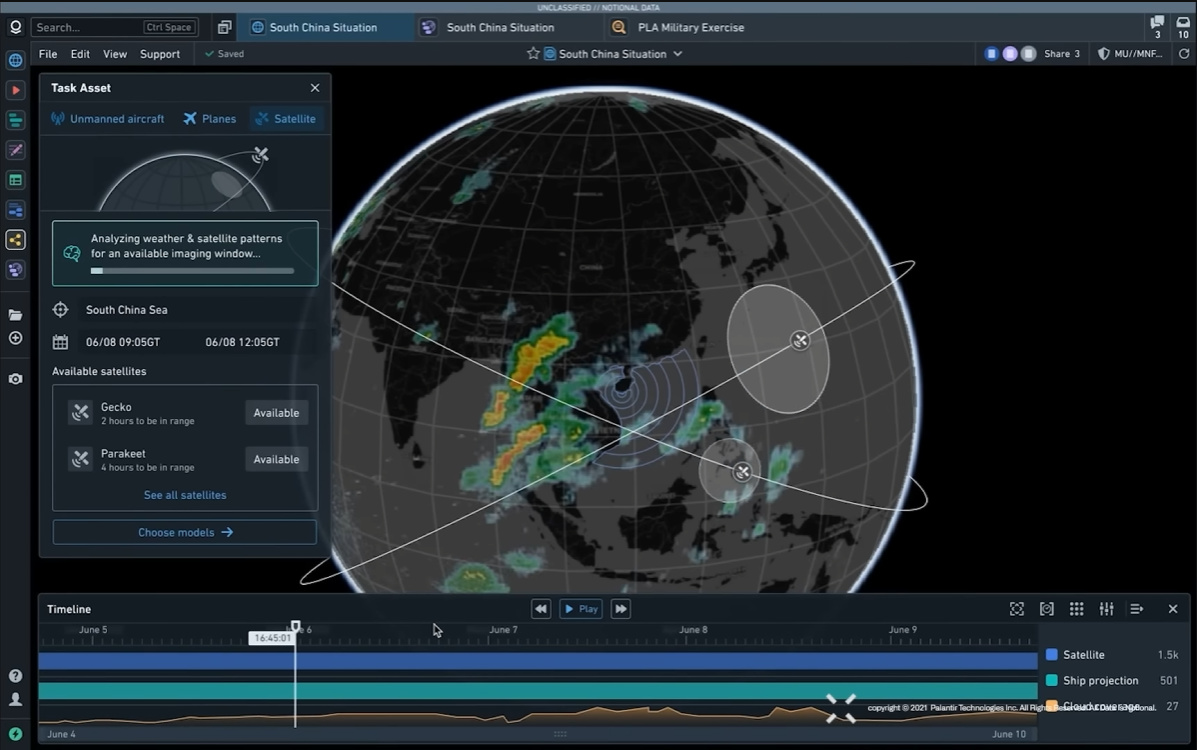
\includegraphics[width=0.85\textwidth]{Photos/Gaia Globalna situaciona svest.jpg}
    \caption{Prikaz centralne Gaia mape koja integriše globalne senzore i satelitske putanje \cite{palantir2021video}.}
    \label{fig:gaia_map}
    \end{figure}
    
    \item \textbf{Graph:} Alat za analizu mreža koji vizuelno prikazuje kako su objekti povezani \cite{wei2024brief}. Na primer, ako operater klikne na određeno vozilo, sistem mu u obliku paukove mreže pokazuje ko je vlasnik, s kim je ta osoba komunicirala i koje je finansijske transakcije obavila \cite{palantir2024gotham}.

    \begin{figure}[H]
    \centering
    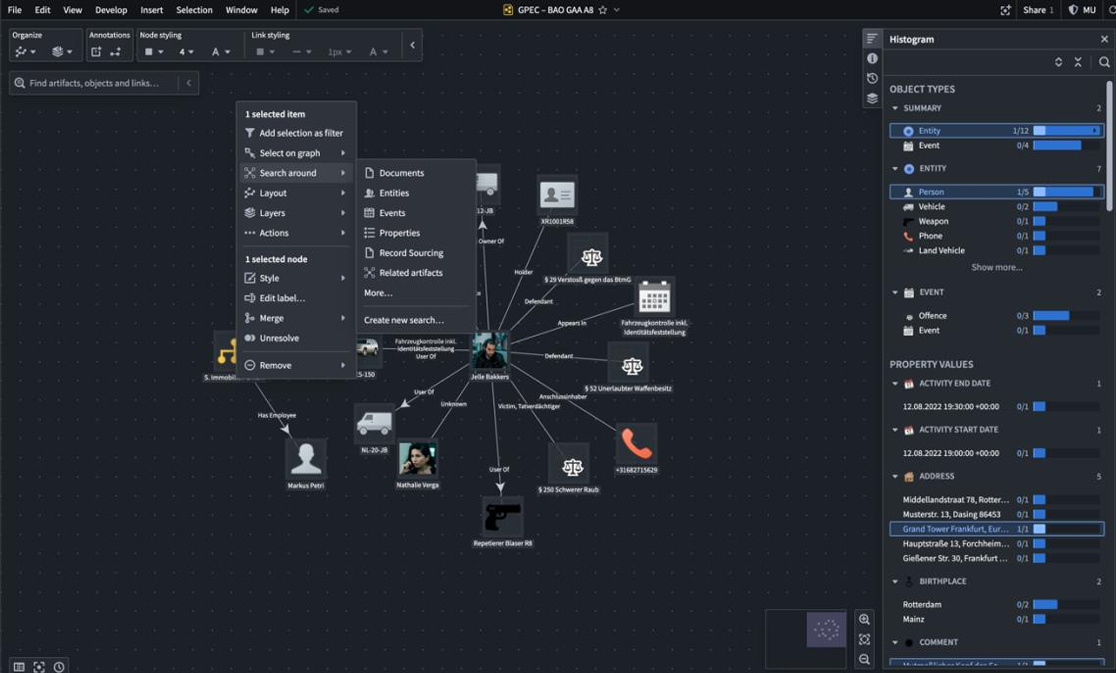
\includegraphics[width=0.85\textwidth]{Photos/Graph Ontologija u praksi.jpg}
    \caption{Vizuelizacija ontologije kroz mrežni graf: povezivanje naizgled nepovezanih entiteta u smislenu celinu \cite{palantir2024gotham}.}
    \label{fig:graph_analiza}
    \end{figure}
    
    \item \textbf{Video:} Alat koji omogućava analizu snimaka sa dronova ili kamera u realnom vremenu, dodajući preko video snimka elemente proširene stvarnosti (AR) \cite{palantir2024gotham}. Operater na živom snimku vidi obeležene zone zabranjenog leta ili identifikovane neprijateljske ciljeve \cite{palantir2024gotham}.

    \begin{figure}[H]
    \centering
    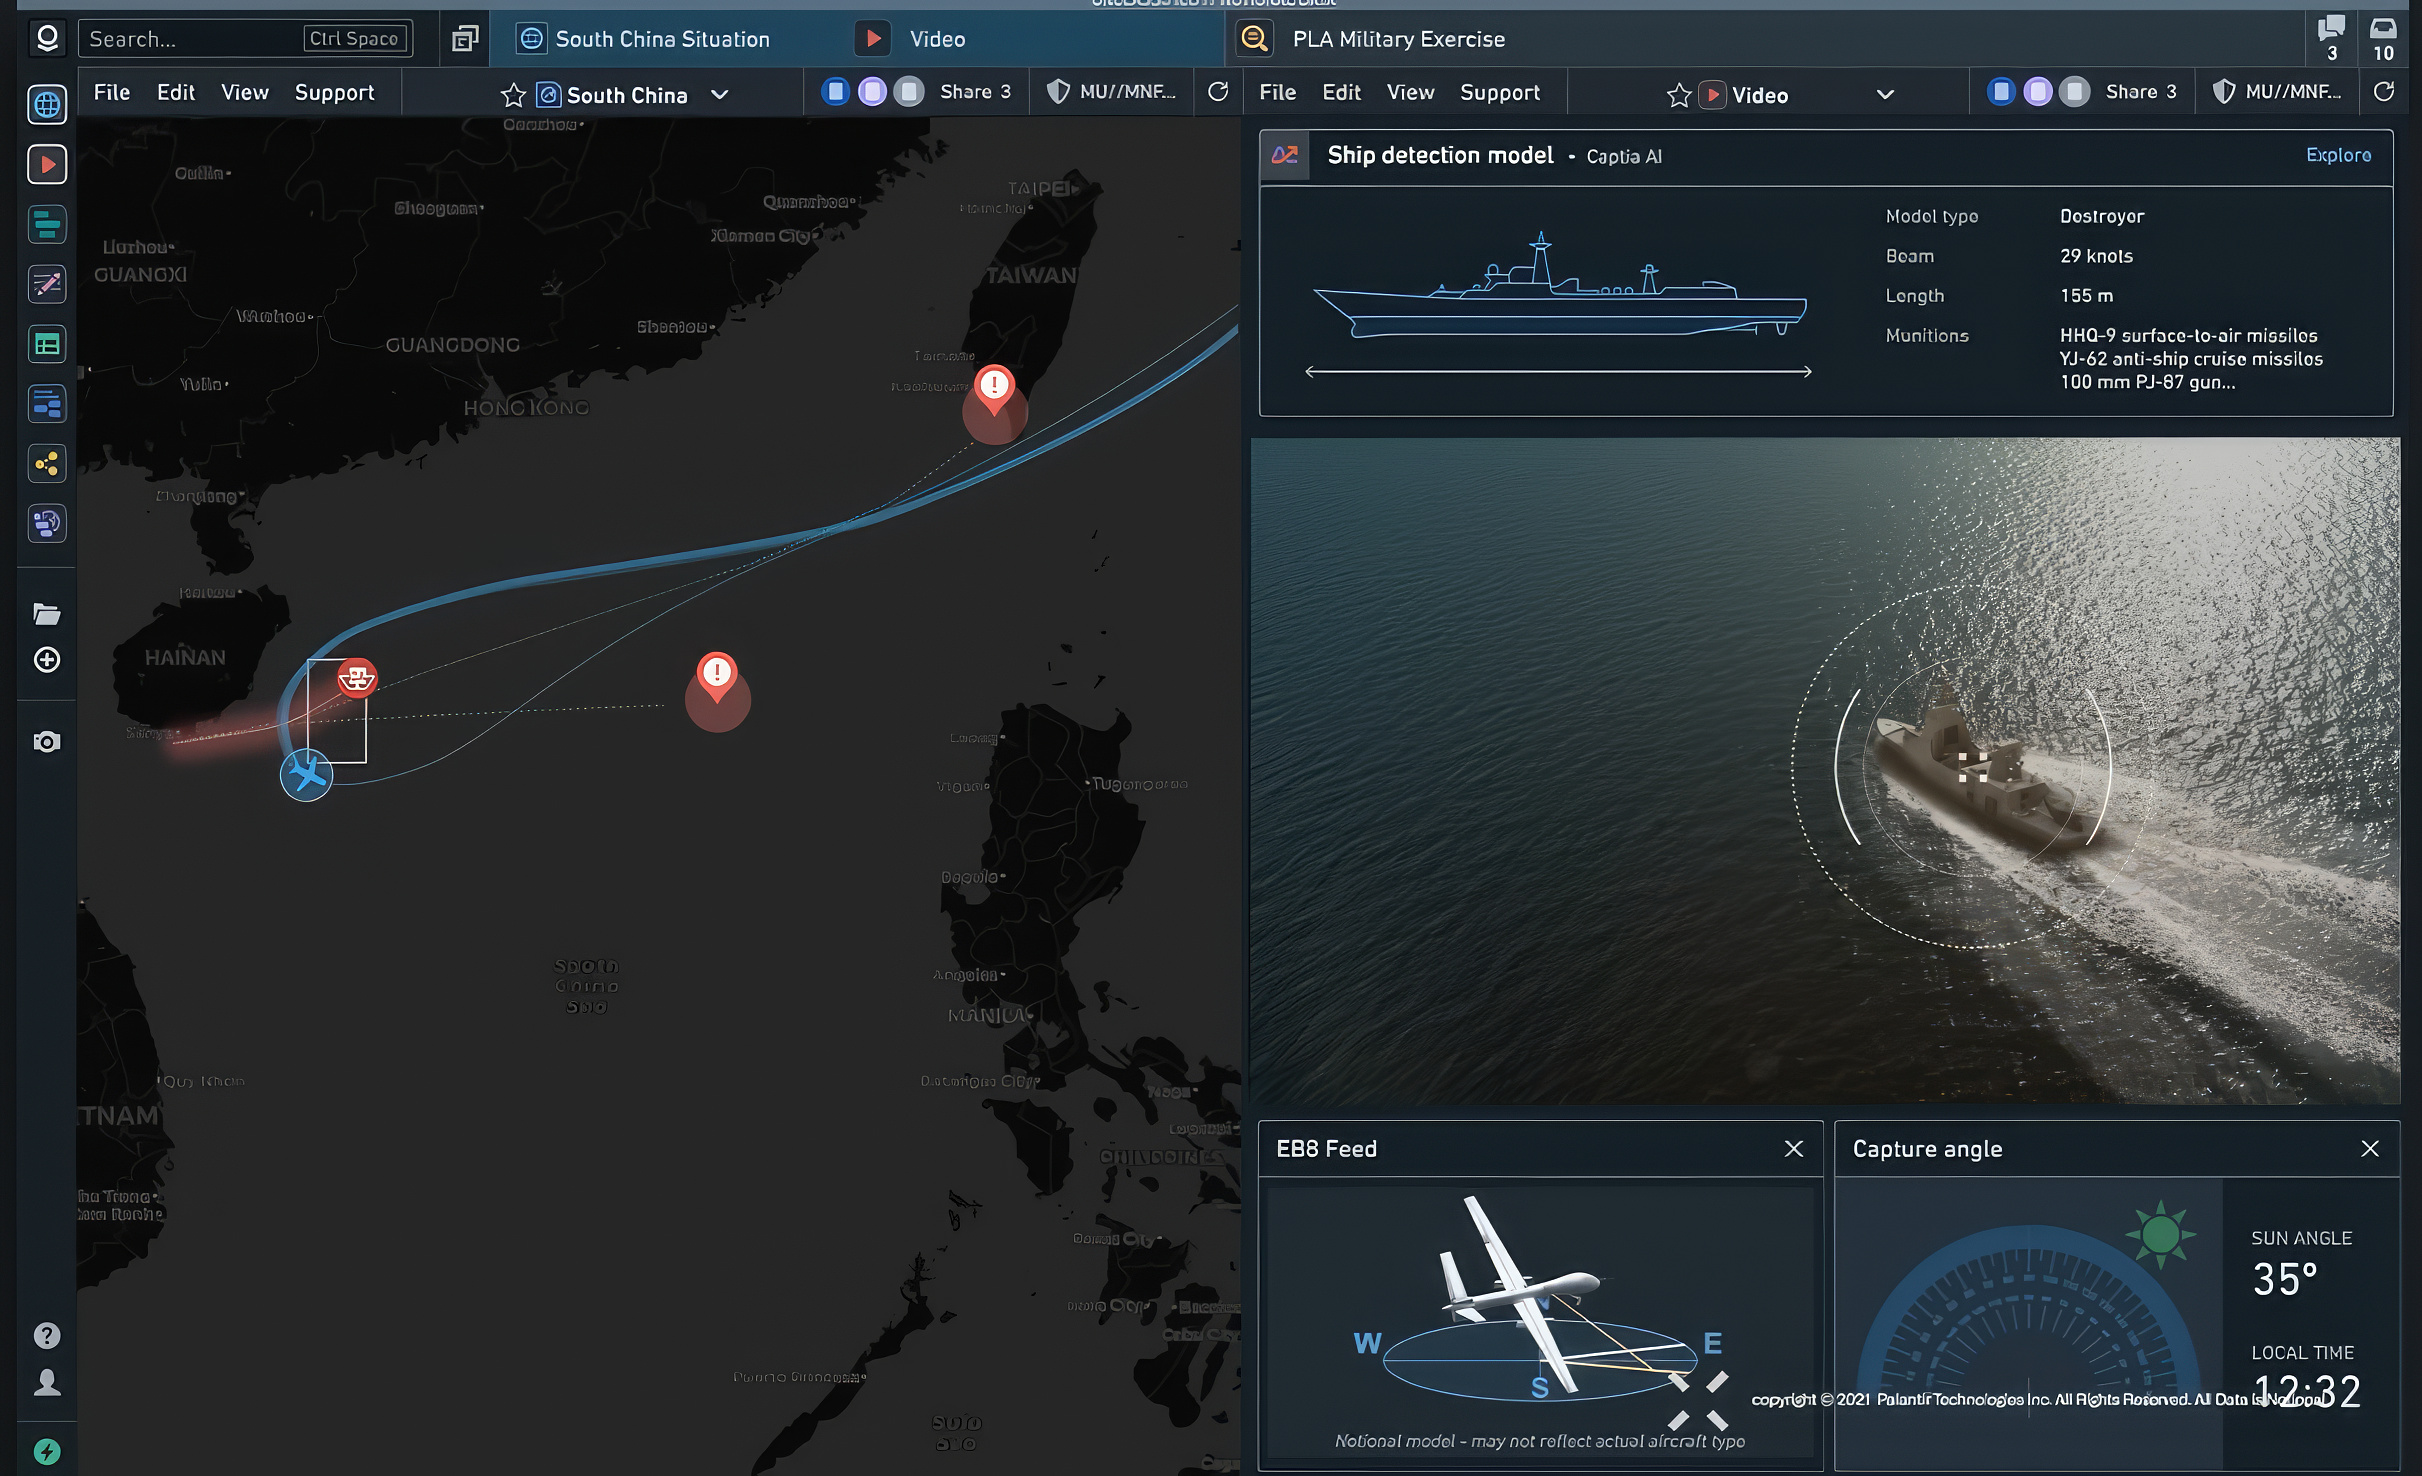
\includegraphics[width=0.85\textwidth]{Photos/Identifikacija objekata pomoću AI.jpg}
    \caption{Automatska klasifikacija i ekstrakcija taktičkih podataka o neprijateljskom brodu pomoću AI modela \cite{palantir2021video}.}
    \label{fig:ai_detekcija}
\end{figure}
    
    \item \textbf{Dossier:} Alat za saradnju sličan pametnom tekstualnom editoru, gde analitičari iz različitih krajeva sveta zajedno pišu izveštaje, prevlačeći (eng. \textit{drag-and-drop}) objekte i mape direktno u tekst, pri čemu podaci ostaju uvek ažurni \cite{wei2024brief, palantir2024gotham}.
\end{itemize}

\begin{figure}[H]
    \centering
    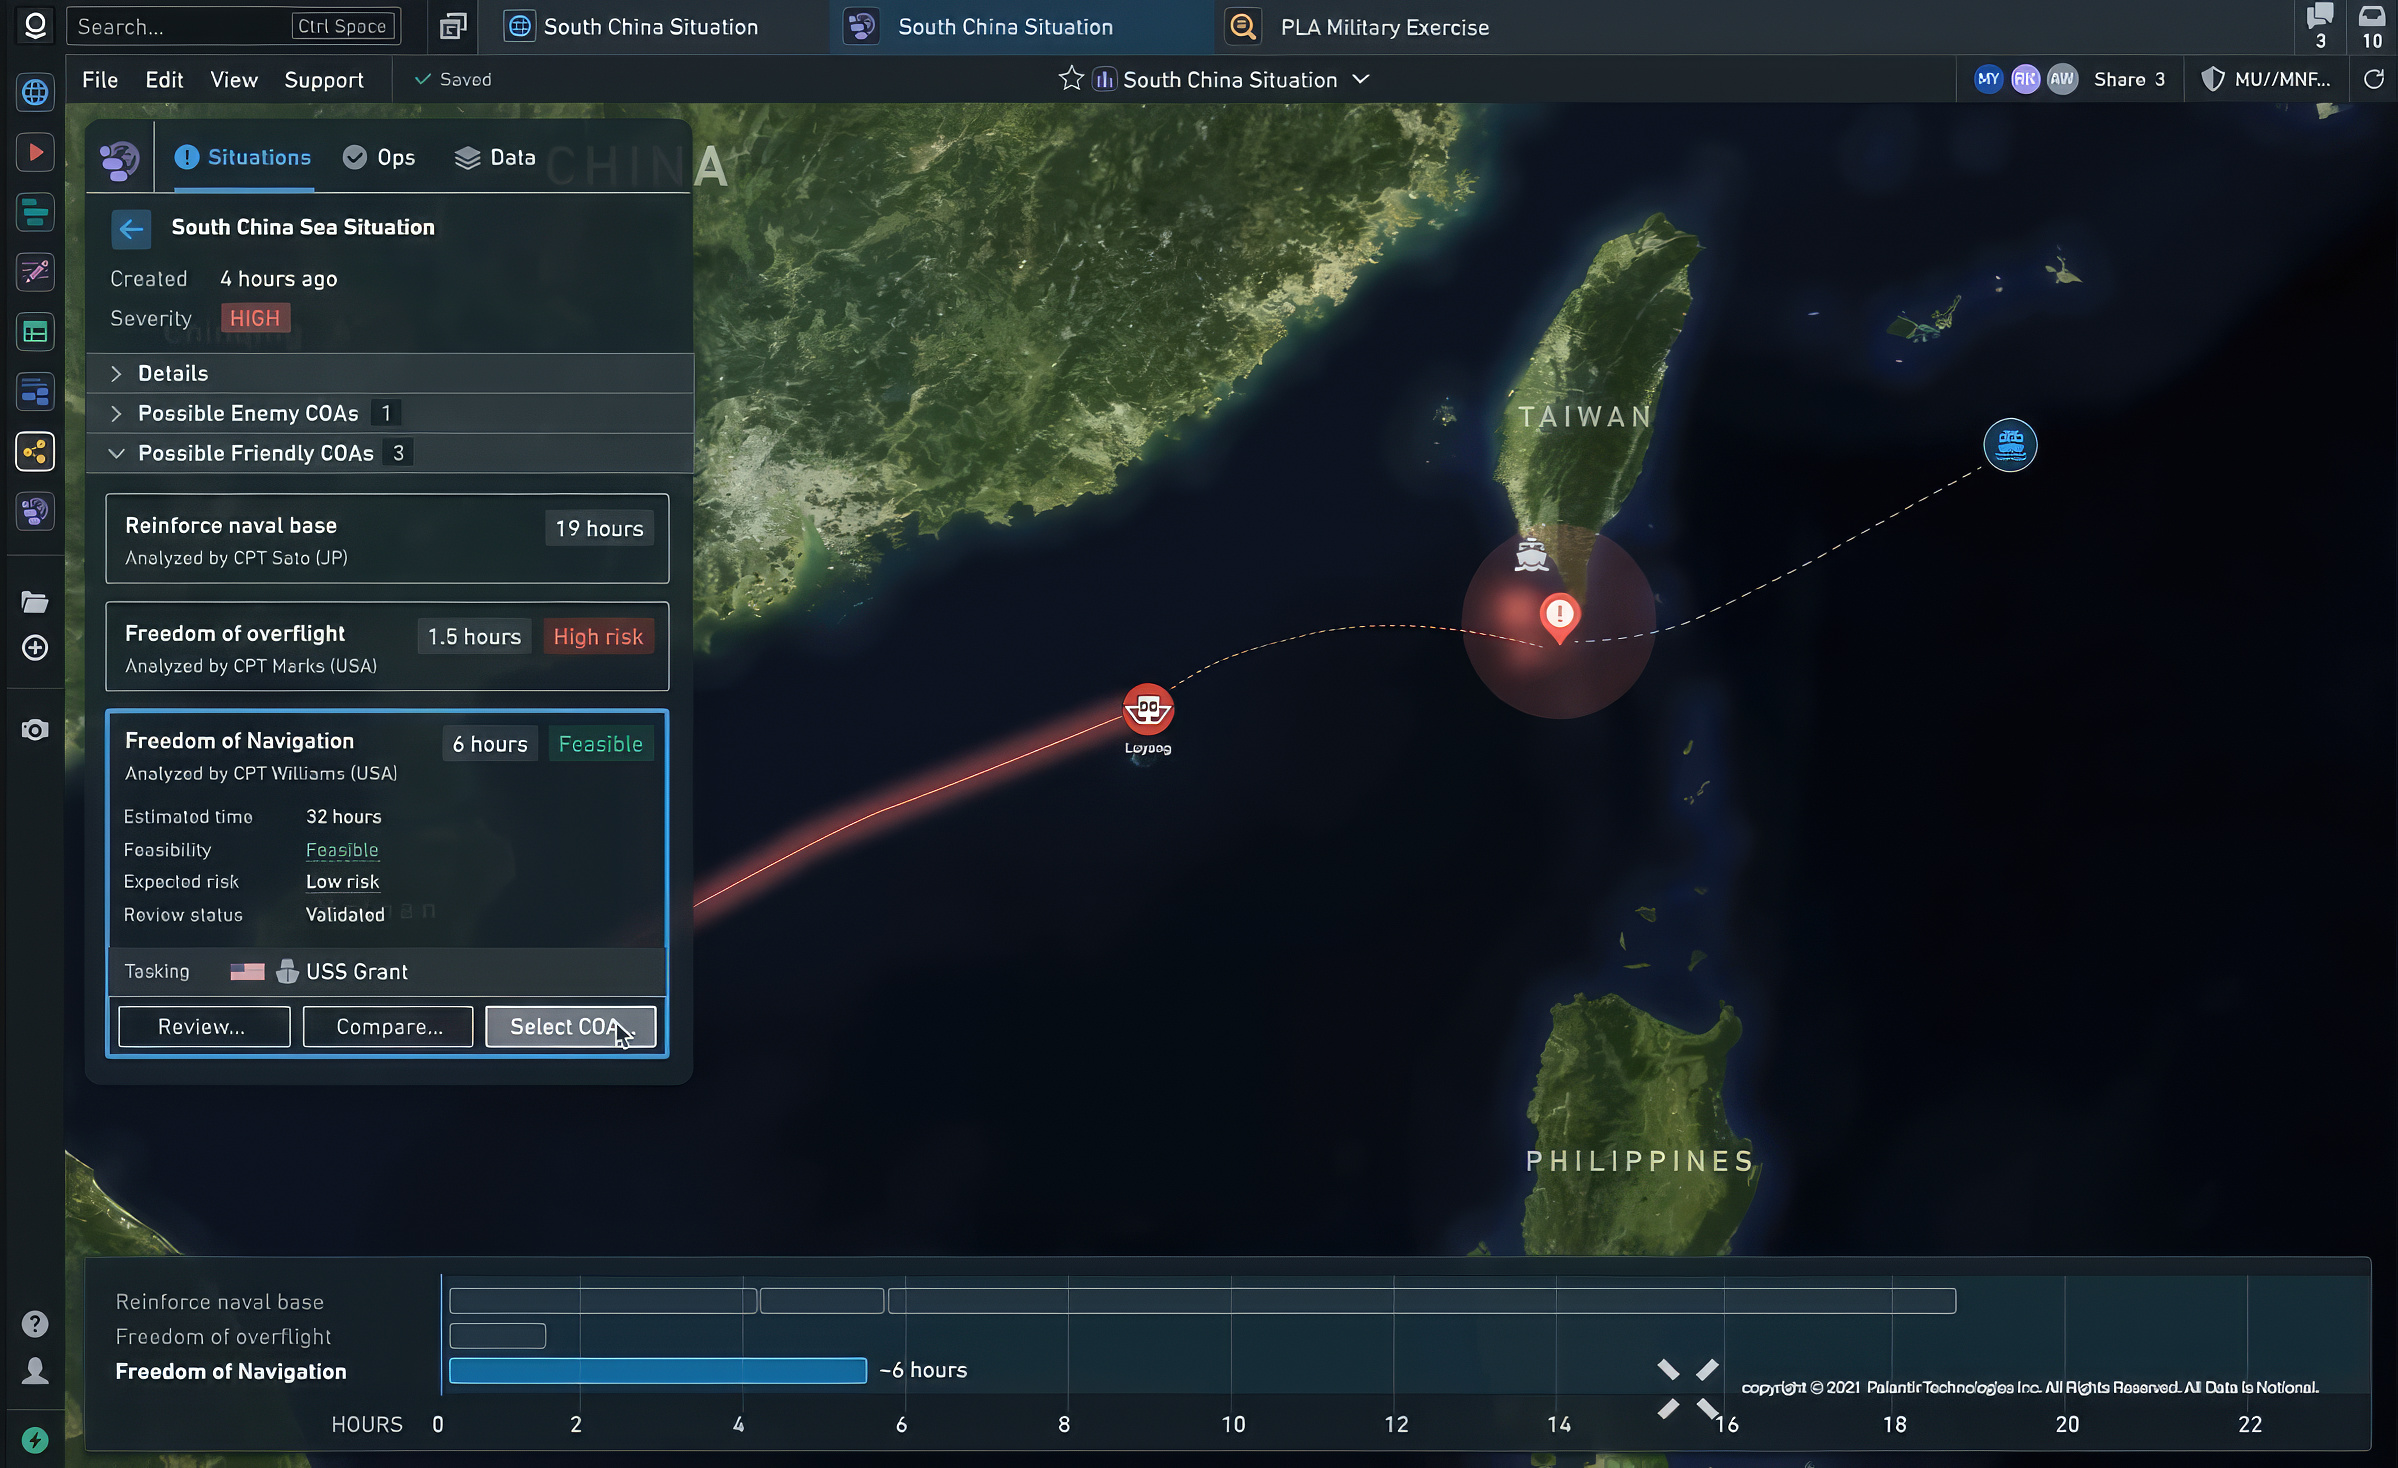
\includegraphics[width=0.85\textwidth]{Photos/Podrška u odlučivanju (COAs) – Most ka Etici.jpg}
    \caption{Algoritamski predlozi različitih kurseva akcije (eng. \textit{Courses of Action - COAs}) sa procenom rizika i efikasnosti \cite{palantir2021video}.}
    \label{fig:decision_support}
\end{figure}

Ovaj sistem omogućava da se tradicionalno spori vojni procesi donošenja odluka, koji su nekada trajali danima, sada kompresuju u svega nekoliko minuta \cite{wei2024brief, woodcock2024human}. Operater više ne mora da pretražuje desetine različitih baza, on sve vidi na jednom ekranu, donoseći odluke intuitivno, klikom na interaktivne elemente \cite{wei2024brief, ulbricht2024palantir}.


\section{Arhitektura sistema Gotham i dinamička ontologija}

Kako bi se razumeo način na koji Gotham obrađuje podatke, neophodno je napraviti otklon od tradicionalnog posmatranja baza podataka. Gotham se ne oslanja na krute šeme tradicionalnih relacionalnih baza (gde se podaci čuvaju u striktno definisanim tabelama), već uvodi koncept poznat kao \textit{dinamička ontologija} \cite{wei2024brief}. 

\subsection{Od sirovih podataka do digitalnog blizanca: Koncept ontologije}

U tradicionalnim relacionim sistemima, manipulacija podacima zahteva direktan rad sa tabelama putem kompleksnih SQL upita i tvrdo kodirane logike (eng. \textit{hardcoded logic}), što od korisnika iziskuje napredne programerske veštine i otežava intuitivno sagledavanje šire slike \cite{wei2024brief}. Problem sa ovakvim statičnim bazama je što se u realnom svetu, posebno u obaveštajnom i bezbednosnom sektoru, podaci stalno menjaju, a nove vrste informacija pristižu u različitim i često nestrukturiranim formatima.

Da bi prevazišao ovo ograničenje, Gotham koristi ontologiju koja suštinski funkcioniše kao napredni graf znanja (eng. \textit{Knowledge Graph}). Ontologija predstavlja digitalnog blizanca stvarnog sveta, gde se svi sirovi podaci iz različitih izvora transformišu i mapiraju u tri osnovna koncepta \cite{wei2024brief}:
\begin{itemize}
    \item \textbf{Objekti (eng. \textit{Objects}):} Predstavljaju stvarne entitete iz fizičkog sveta, kao što su osobe, vozila, zgrade, oružje ili čak događaji i nestrukturirani dokumenti.
    \item \textbf{Svojstva (eng. \textit{Properties}):} Predstavljaju atribute koji opisuju objekte (npr. ime i prezime osobe, registarski broj vozila ili datum rođenja).
    \item \textbf{Veze (eng. \textit{Links}):} Predstavljaju relacije između objekata (npr. veza \enquote{je vlasnik} između objekta \textit{Osoba} i objekta \textit{Vozilo}).
\end{itemize}

Ovakva arhitektura vođena grafovima omogućava da se umesto pretrage po izolovanim tabelama, podaci pretražuju i vizuelno analiziraju kroz mrežu međusobno povezanih čvorova (objekata) i grana (veza). Na ovaj način, kompleksni odnosi između naizgled nepovezanih informacija postaju očigledni, a analitičari mogu da istražuju podatke vođeni čistom poslovnom logikom, a ne tehničkom strukturom same baze \cite{wei2024brief}.

\subsection{Dinamička priroda ontologije (Semantički, Kinetički i Dinamički sloj)}

Ključni inženjerski problem kod tradicionalnih arhitektura je taj što promena šeme baze podataka ili ažuriranje složenih relacija u hodu zahteva ozbiljne intervencije i programersko znanje (npr. pisanje kompleksnih SQL \textit{UPDATE} upita). Na modernom bojištu ili u središtu obaveštajne operacije, podaci se menjaju iz sekunde u sekundu, pa statične šeme jednostavno nisu upotrebljive.

Kako bi rešio ovaj problem, Palantir umesto tradicionalnih manipulacija podacima uvodi koncept takozvanih \textit{Action Types} (tipova akcija) \cite{wei2024brief}. Kroz grafički interfejs, analitičar može intuitivno da izmeni svojstvo nekog objekta ili doda novu vezu, a sistem u pozadini samostalno generiše i sprovodi neophodne logičke operacije nad bazom. Da bi ovo funkcionisalo, dinamička ontologija je podeljena u tri funkcionalna sloja \cite{wei2024brief}:

\begin{itemize}
    \item \textbf{Semantički sloj (eng. \textit{Semantic Layer}):} Ovo je osnovni sloj u kom se sirovi podaci mapiraju u ranije pomenute objekte i veze. Ovaj sloj takođe obezbeđuje i najsitnije kontrole pristupa, osiguravajući da svaki korisnik vidi samo one objekte i svojstva za koje ima eksplicitno odobrenje (tzv. \textit{Purpose Based Access Controls}).
    \item \textbf{Kinetički sloj (eng. \textit{Kinetic Layer}):} Služi za modelovanje poslovnih procesa i orkestraciju. On hvata sve promene koje korisnici prave i na osnovu njih automatski pokreće algoritme veštačke inteligencije (AI) ili druge funkcije u pozadini, čime se sistem neprestano prilagođava novim podacima.
    \item \textbf{Dinamički sloj (eng. \textit{Dynamic Layer}):} Ovo je vrhunac arhitekture koji duboko integriše ontologiju sa vizuelnim front-end aplikacijama. Omogućava donošenje odluka potpomognutih veštačkom inteligencijom, hvatanje korisničkih odluka, kao i pokretanje višestepenih simulacija na osnovu trenutnog stanja ontologije.
\end{itemize}

Ovaj pristup omogućava da sistem prestane da bude samo pasivno skladište informacija i postane živi digitalni blizanac realnog okruženja, koji se iz sekunde u sekundu ažurira zajedničkim naporom ljudskih analitičara i mašinskih algoritama \cite{wei2024brief}.

\subsection{Razrešavanje entiteta (Entity Resolution)}

Kada integrišemo ogromne količine sirovih podataka iz različitih izvora, javlja se jedan od najvećih problema u nauci o podacima: kako sistem zna da su \enquote{P. Perić} iz baze saobraćajne policije i \enquote{PeraPerich04} sa nekog internet foruma zapravo ista osoba u realnom svetu? 
Proces koji rešava ovaj problem naziva se razrešavanje entiteta (eng. \textit{Entity Resolution - ER}) \cite{architecture2024}. Bez visoko preciznog ER-a, naša ontologija bi bila prepuna duplikata i nepovezanih čvorova, što bi dovelo do potpuno pogrešnih analitičkih zaključaka.

Tradicionalne relacione baze se za spajanje zapisa obično oslanjaju na strogo poklapanje (eng. \textit{exact-match blocking}), na primer poklapanje jedinstvenog matičnog broja ili tačnog imena. Međutim, u bezbednosnom sektoru podaci su često nepotpuni, puni šuma ili slovnih grešaka. Gotham ovom problemu pristupa korišćenjem sofisticiranih algoritama baziranih na potpisima i verovatnoći \cite{architecture2024}.

Sistem analizira podatke tražeći takozvane \enquote{potpise} (eng. \textit{signatures}) - podzapise ili kombinacije atributa koje su statistički jedinstvene za neki entitet \cite{architecture2024}. Na primer, često ime poput \enquote{Jovan Jovanović} nije dobar potpis, ali kombinacija tog imena, specifične ulice i modela automobila ima visoku verovatnoću da jedinstveno identifikuje osobu. Ovaj algoritamski proces u Gothamu se odvija kroz nekoliko ključnih inženjerskih koraka \cite{architecture2024}:

\begin{itemize}
    \item \textbf{Generisanje obrnutog indeksa (eng. \textit{Inverted Index}):} Sistem prvo indeksira sve podzapise i računa koliko se često pojavljuju. Ovo omogućava algoritmu da nauči kako da razlikuje unikatne statističke potpise od uobičajenog šuma u podacima.
    \item \textbf{Probabilističko blokiranje (eng. \textit{Probabilistic Blocking}):} Umesto striktnog poređenja karaktera u kolonama, sistem formira \enquote{blokove} za poređenje koristeći verovatnoće. Na ovaj način algoritam sužava pretragu i uspešno pronalazi veze čak i kada postoje slovne greške u imenima ili delimično izmenjene adrese.
    \item \textbf{Tranzitivno povezivanje (eng. \textit{Transitive Linkage}):} Obaveštajni podaci su često poput paukove mreže indirektnih veza. Algoritam koristi teoriju grafova, tačnije pronalaženje komponenti povezanosti (eng. \textit{connected components}). Ako postoji verovatnoća poklapanja zapisa A sa zapisom B, kao i zapisa B sa zapisom C, sistem će automatski dodeliti isti identifikator za sva tri zapisa, čak i ako Zapisi A i C nemaju nijedan direktno zajednički atribut.
\end{itemize}

Zahvaljujući ovom pristupu, Gotham omogućava da se milijarde sirovih i neurednih zapisa automatski pročiste i spoje u jedinstvene objekte. Ovo arhitekturi omogućava linearno skaliranje i brzu obradu podataka na nivou celokupnog državnog aparata \cite{architecture2024}.

\subsection{Reviziona baza podataka (RevDB) i nedestruktivno spajanje}

Iako algoritmi za razrešavanje entiteta postižu visoku preciznost, uvek postoji mogućnost greške (npr. spajanje dve različite osobe sa istim imenom u jedan entitet). U tradicionalnim relacionim bazama, operacije spajanja (eng. \textit{merge}) često nepovratno prepisuju ili brišu originalne podatke. Za razliku od toga, proces razrešavanja entiteta u sistemu Gotham je potpuno nedestruktivan \cite{architecture2024}.

Palantir ovaj problem rešava implementacijom Revizione baze podataka (eng. \textit{Revision Database - RevDB}). Svaka akcija spajanja entiteta u ontologiji se ne tretira kao prepisivanje podataka, već se beleži kao nova transakcija unutar RevDB-a \cite{architecture2024}. Zahvaljujući ovom mehanizmu, sistem čuva kompletno poreklo svakog pojedinačnog zapisa (eng. \textit{data lineage}). 

Ukoliko analitičar ili sam algoritam naknadno utvrdi da je došlo do greške i da dva spojena zapisa zapravo ne predstavljaju isti objekat u realnom svetu, RevDB omogućava jednostavno \enquote{rasparčavanje} (eng. \textit{unresolve}) entiteta \cite{architecture2024}. Sistem tada automatski vraća podatke u njihovo prvobitno stanje, bez ikakvog gubitka informacija.

Ovakva arhitektura je od presudnog značaja ne samo iz tehničkog, već i iz pravnog i etičkog ugla. RevDB osigurava potpunu transparentnost i reviziju (eng. \textit{auditability}) svih aktivnosti u sistemu \cite{architecture2024}. U osetljivim vojnim i policijskim operacijama, ovo omogućava nadležnim organima da u svakom trenutku jasno utvrde na osnovu kojih tačno izvornih podataka i čijom odlukom je sprovedena određena akcija na terenu.

\section{Etika u vojnoj primeni i problem čoveka u petlji}

Integracija sistema kao što je Palantir Gotham u vojnu sferu donosi sa sobom fundamentalna etička pitanja koja prevazilaze čiste inženjerske performanse. Glavni izazov leži u tome kako zadržati kontrolu nad procesima koji se odvijaju brzinom i kompleksnošću koju ljudski mozak ne može u potpunosti da prati.

\subsection{Koncept „suštinska ljudska kontrola” (Meaningful Human Control)}

U diskusijama o vojnoj primeni veštačke inteligencije, često se ističe da čovek mora ostati \textit{u petlji} (eng. \textit{Human-in-the-Loop}), odnosno da mora biti jedini i konačni donosilac odluka \cite{woodcock2024human, ethical2025reconnaissance}. Međutim, u praksi sa Gothamom, postavlja se pitanje da li je to prisustvo čoveka suštinsko ili samo formalno.

Koncept \textit{suštinske ljudske kontrole} podrazumeva da operater ne sme biti samo \enquote{gumeni pečat} (eng. \textit{rubber stamp}) za odluke koje je sistem već pripremio \cite{ethical2025reconnaissance}. Da bi kontrola bila stvarna, proces rada softvera mora biti potpuno transparentan (eng. \textit{traceable}), korisnik mora razumeti ne samo konačni rezultat, već i svaki korak koji je sistem napravio da bi do tog rezultata došao \cite{ethical2025reconnaissance, architecture2024}. 

Na slici \ref{fig:decision_support} videli smo da Gotham nudi tri Kursa Akcije (COAs) sa procenjenim rizikom. Ukoliko operater, pod pritiskom vremena, uvek bira opciju označenu kao \enquote{Low Risk}, on suštinski prepušta odluku algoritmu. U tom scenariju, sposobnost čoveka da samostalno donosi odluke biva potisnuta u korist algoritamske logike koja prioritet daje brzini i efikasnosti umesto dubokom moralnom rasuđivanju \cite{woodcock2024human, tilbury2024automation}.

\subsection{Automation Bias: Zamka nepogrešivosti algoritma}

Jedan od najopasnijih psiholoških i tehničkih fenomena u radu sa Gothamom je \textit{automation bias}, ljudska sklonost da se slepo veruje automatizovanim sistemima, čak i kada oni daju netačne informacije \cite{tilbury2024automation}. 

Ovaj problem je dodatno naglašen zbog tri ključna faktora:
\begin{itemize}
    \item \textbf{Kognitivno zabušavanje (eng. \textit{Cognitive social loafing}):} Operateri podsvesno ulažu manje truda u proveru podataka jer pretpostavljaju da je softver već obradio milijarde informacija nepogrešivo \cite{tilbury2024automation}.
    \item \textbf{Problem crne kutije:} Algoritmi dubokog učenja su često nečitljivi (\textit{inscrutable}). Čak i ako operater želi da proveri odluku, on ne može da vidi unutrašnju logiku kojom je mašina procesirala Big Data setove u realnom vremenu \cite{woodcock2024human}.
    \item \textbf{Pritisak vremena:} Brzina kojom Gotham obrađuje podatke tera ljude da vrednuju brzo reagovanje više nego traženje informacija koje bi mogle da opovrgnu preporuku sistema \cite{tilbury2024automation}.
\end{itemize}

U bezbednosnom kontekstu, ovo stvara lažni osećaj sigurnosti. Ako sistem greškom spoji dva entiteta u jedan, a analitičar to ne proveri zbog poverenja u sistem, posledice na terenu mogu biti fatalne \cite{tilbury2024automation, ethical2025reconnaissance}.

\subsection{Algoritamska pristrasnost i problem „targetiranja”}

Iako se algoritmi često promovišu kao objektivni, oni su zapravo ogledalo podataka na kojima su trenirani. Algoritamska pristrasnost (eng. \textit{algorithmic bias}) u sistemu kao što je Gotham može se javiti u tri oblika: kroz pristrasne ulazne podatke, tehnički dizajn samog modela ili kroz način na koji korisnici interpretiraju rezultate \cite{icrc2024bias}.

Jedan od najvećih rizika je takozvana \textit{uzorkovana pristrasnost} (eng. \textit{sampling bias}). Ukoliko su podaci za obuku Gothama prikupljani u specifičnim demografskim zonama, sistem može razviti nepravilne obrasce identifikacije \cite{icrc2024bias}. U kontekstu modernog ratovanja, gde Palantir promoviše \enquote{AI-vođeni lanac targetiranja} (eng. \textit{AI-powered kill chain}), ovo može dovesti do tragičnih posledica \cite{carnegie2024private}. Ako sistem na osnovu istorijskih podataka određene grupe ljudi ili tipove ponašanja češće označava kao pretnju, operater može dobiti lažno potvrđenu metu, što direktno vodi ka diskriminatornim ishodima na terenu \cite{icrc2024bias, carnegie2024private}.

\subsection{Problem proporcionalnosti: Može li AI da vrednuje ljudski život?}

Prema Međunarodnom humanitarnom pravu, svaka vojna odluka mora da zadovolji princip proporcionalnosti - odmeravanje očekivane vojne prednosti u odnosu na potencijalni rizik po civilno stanovništvo \cite{woodcock2024human, icrc2024bias}. Ovde nastaje fundamentalni inženjerski i etički problem: proporcionalnost zahteva \textit{vrednosni sud}, a ne samo matematičku kalkulaciju \cite{woodcock2024human}.

Softver kao što je Gotham operiše u domenu verovatnoće i brojeva. On može da izračuna radijus eksplozije ili proceni broj objekata u zoni, ali nije sposoban da razume moralnu težinu gubitka ljudskog života \cite{woodcock2024human, hua2020rethinking}. Problem \enquote{crne kutije} ovde postaje kritičan. Pošto su algoritmi mašinskog učenja često neprozirni, komandant ne može pravno niti moralno da opravda zašto je sistem procenio da je određena žrtva \enquote{proporcionalna} cilju \cite{woodcock2024human, icrc2024bias}. Autorka Taylor Woodcock naglašava da su zbog ove nečitljivosti AI sistemi suštinski neadekvatni za samostalno donošenje ovakvih odluka \cite{woodcock2024human}.

\subsection{Jaz u odgovornosti (Accountability Gap)}

Na kraju, postavlja se ključno pitanje: ko snosi odgovornost kada Gotham pogreši? Integracija privatnih tehnoloških kompanija u državni aparat stvara opasan \textit{jaz u odgovornosti} \cite{carnegie2024private, architecture2024}. U ovom trouglu moći: država, privatna kompanija i operater - odgovornost postaje nejasna \cite{carnegie2024private, ulbricht2024palantir}.

\begin{itemize}
    \item \textbf{Država} može tvrditi da je koristila softver koji je \enquote{proveren i licenciran}.
    \item \textbf{Kompanija (Palantir)} može tvrditi da je softver samo \enquote{alat za podršku}, a da je konačnu odluku doneo čovek.
    \item \textbf{Operater} se može braniti time da je samo pratio preporuku sistema koju nije mogao samostalno da proveri zbog složenosti Big Data analitike \cite{carnegie2024private, ulbricht2024palantir}.
\end{itemize}

Ovaj informacioni jaz između onih koji prave softver i onih koji ga koriste dovodi do situacije u kojoj se suvereni državni autoritet (pravo na upotrebu sile) prenosi na zatvorene algoritme privatnih korporacija, čime se direktno ugrožava demokratski nadzor i vladavina prava \cite{carnegie2024private, ulbricht2024palantir, architecture2024}.

\section{Problem privatnosti, nadzora i bezbednosti interneta}


\section{Zaključak}

\newpage
\printbibliography

\end{document}